\documentclass[1p]{elsarticle_modified}
%\bibliographystyle{elsarticle-num}

%\usepackage[colorlinks]{hyperref}
%\usepackage{abbrmath_seonhwa} %\Abb, \Ascr, \Acal ,\Abf, \Afrak
\usepackage{amsfonts}
\usepackage{amssymb}
\usepackage{amsmath}
\usepackage{amsthm}
\usepackage{scalefnt}
\usepackage{amsbsy}
\usepackage{kotex}
\usepackage{caption}
\usepackage{subfig}
\usepackage{color}
\usepackage{graphicx}
\usepackage{xcolor} %% white, black, red, green, blue, cyan, magenta, yellow
\usepackage{float}
\usepackage{setspace}
\usepackage{hyperref}

\usepackage{tikz}
\usetikzlibrary{arrows}

\usepackage{multirow}
\usepackage{array} % fixed length table
\usepackage{hhline}

%%%%%%%%%%%%%%%%%%%%%
\makeatletter
\renewcommand*\env@matrix[1][\arraystretch]{%
	\edef\arraystretch{#1}%
	\hskip -\arraycolsep
	\let\@ifnextchar\new@ifnextchar
	\array{*\c@MaxMatrixCols c}}
\makeatother %https://tex.stackexchange.com/questions/14071/how-can-i-increase-the-line-spacing-in-a-matrix
%%%%%%%%%%%%%%%

\usepackage[normalem]{ulem}

\newcommand{\msout}[1]{\ifmmode\text{\sout{\ensuremath{#1}}}\else\sout{#1}\fi}
%SOURCE: \msout is \stkout macro in https://tex.stackexchange.com/questions/20609/strikeout-in-math-mode

\newcommand{\cancel}[1]{
	\ifmmode
	{\color{red}\msout{#1}}
	\else
	{\color{red}\sout{#1}}
	\fi
}

\newcommand{\add}[1]{
	{\color{blue}\uwave{#1}}
}

\newcommand{\replace}[2]{
	\ifmmode
	{\color{red}\msout{#1}}{\color{blue}\uwave{#2}}
	\else
	{\color{red}\sout{#1}}{\color{blue}\uwave{#2}}
	\fi
}

\newcommand{\Sol}{\mathcal{S}} %segment
\newcommand{\D}{D} %diagram
\newcommand{\A}{\mathcal{A}} %arc


%%%%%%%%%%%%%%%%%%%%%%%%%%%%%5 test

\def\sl{\operatorname{\textup{SL}}(2,\Cbb)}
\def\psl{\operatorname{\textup{PSL}}(2,\Cbb)}
\def\quan{\mkern 1mu \triangleright \mkern 1mu}

\theoremstyle{definition}
\newtheorem{thm}{Theorem}[section]
\newtheorem{prop}[thm]{Proposition}
\newtheorem{lem}[thm]{Lemma}
\newtheorem{ques}[thm]{Question}
\newtheorem{cor}[thm]{Corollary}
\newtheorem{defn}[thm]{Definition}
\newtheorem{exam}[thm]{Example}
\newtheorem{rmk}[thm]{Remark}
\newtheorem{alg}[thm]{Algorithm}

\newcommand{\I}{\sqrt{-1}}
\begin{document}

%\begin{frontmatter}
%
%\title{Boundary parabolic representations of knots up to 8 crossings}
%
%%% Group authors per affiliation:
%\author{Yunhi Cho} 
%\address{Department of Mathematics, University of Seoul, Seoul, Korea}
%\ead{yhcho@uos.ac.kr}
%
%
%\author{Seonhwa Kim} %\fnref{s_kim}}
%\address{Center for Geometry and Physics, Institute for Basic Science, Pohang, 37673, Korea}
%\ead{ryeona17@ibs.re.kr}
%
%\author{Hyuk Kim}
%\address{Department of Mathematical Sciences, Seoul National University, Seoul 08826, Korea}
%\ead{hyukkim@snu.ac.kr}
%
%\author{Seokbeom Yoon}
%\address{Department of Mathematical Sciences, Seoul National University, Seoul, 08826,  Korea}
%\ead{sbyoon15@snu.ac.kr}
%
%\begin{abstract}
%We find all boundary parabolic representation of knots up to 8 crossings.
%
%\end{abstract}
%\begin{keyword}
%    \MSC[2010] 57M25 
%\end{keyword}
%
%\end{frontmatter}

%\linenumbers
%\tableofcontents
%
\newcommand\colored[1]{\textcolor{white}{\rule[-0.35ex]{0.8em}{1.4ex}}\kern-0.8em\color{red} #1}%
%\newcommand\colored[1]{\textcolor{white}{ #1}\kern-2.17ex	\textcolor{white}{ #1}\kern-1.81ex	\textcolor{white}{ #1}\kern-2.15ex\color{red}#1	}

{\Large $\underline{12n_{0206}~(K12n_{0206})}$}

\setlength{\tabcolsep}{10pt}
\renewcommand{\arraystretch}{1.6}
\vspace{1cm}\begin{tabular}{m{100pt}>{\centering\arraybackslash}m{274pt}}
\multirow{5}{120pt}{
	\centering
	\includegraphics[width=112pt]{../../../GIT/diagram.site/Diagrams/png/2295_12n_0206.png}\\
\ \ \ A knot diagram\footnotemark}&
\allowdisplaybreaks
\textbf{Linearized knot diagam} \\
\cline{2-2}
 &
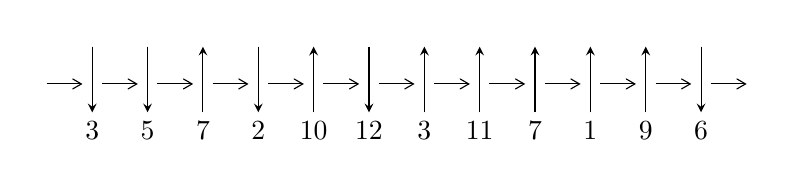
\begin{tikzpicture}[x=20pt, y=17pt]
	% nodes
	\node (C0) at (0, 0) {};
	\node (C1) at (1, 0) {};
	\node (C1U) at (1, +1) {};
	\node (C1D) at (1, -1) {3};

	\node (C2) at (2, 0) {};
	\node (C2U) at (2, +1) {};
	\node (C2D) at (2, -1) {5};

	\node (C3) at (3, 0) {};
	\node (C3U) at (3, +1) {};
	\node (C3D) at (3, -1) {7};

	\node (C4) at (4, 0) {};
	\node (C4U) at (4, +1) {};
	\node (C4D) at (4, -1) {2};

	\node (C5) at (5, 0) {};
	\node (C5U) at (5, +1) {};
	\node (C5D) at (5, -1) {10};

	\node (C6) at (6, 0) {};
	\node (C6U) at (6, +1) {};
	\node (C6D) at (6, -1) {12};

	\node (C7) at (7, 0) {};
	\node (C7U) at (7, +1) {};
	\node (C7D) at (7, -1) {3};

	\node (C8) at (8, 0) {};
	\node (C8U) at (8, +1) {};
	\node (C8D) at (8, -1) {11};

	\node (C9) at (9, 0) {};
	\node (C9U) at (9, +1) {};
	\node (C9D) at (9, -1) {7};

	\node (C10) at (10, 0) {};
	\node (C10U) at (10, +1) {};
	\node (C10D) at (10, -1) {1};

	\node (C11) at (11, 0) {};
	\node (C11U) at (11, +1) {};
	\node (C11D) at (11, -1) {9};

	\node (C12) at (12, 0) {};
	\node (C12U) at (12, +1) {};
	\node (C12D) at (12, -1) {6};
	\node (C13) at (13, 0) {};

	% arrows
	\draw[->,>={angle 60}]
	(C0) edge (C1) (C1) edge (C2) (C2) edge (C3) (C3) edge (C4) (C4) edge (C5) (C5) edge (C6) (C6) edge (C7) (C7) edge (C8) (C8) edge (C9) (C9) edge (C10) (C10) edge (C11) (C11) edge (C12) (C12) edge (C13) ;	\draw[->,>=stealth]
	(C1U) edge (C1D) (C2U) edge (C2D) (C3D) edge (C3U) (C4U) edge (C4D) (C5D) edge (C5U) (C6U) edge (C6D) (C7D) edge (C7U) (C8D) edge (C8U) (C9D) edge (C9U) (C10D) edge (C10U) (C11D) edge (C11U) (C12U) edge (C12D) ;
	\end{tikzpicture} \\
\hhline{~~} \\& 
\textbf{Solving Sequence} \\ \cline{2-2} 
 &
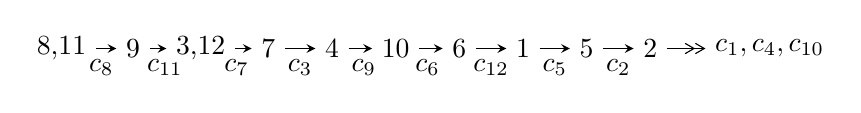
\begin{tikzpicture}[x=23pt, y=7pt]
	% node
	\node (A0) at (-1/8, 0) {8,11};
	\node (A1) at (1, 0) {9};
	\node (A2) at (33/16, 0) {3,12};
	\node (A3) at (25/8, 0) {7};
	\node (A4) at (33/8, 0) {4};
	\node (A5) at (41/8, 0) {10};
	\node (A6) at (49/8, 0) {6};
	\node (A7) at (57/8, 0) {1};
	\node (A8) at (65/8, 0) {5};
	\node (A9) at (73/8, 0) {2};
	\node (C1) at (1/2, -1) {$c_{8}$};
	\node (C2) at (3/2, -1) {$c_{11}$};
	\node (C3) at (21/8, -1) {$c_{7}$};
	\node (C4) at (29/8, -1) {$c_{3}$};
	\node (C5) at (37/8, -1) {$c_{9}$};
	\node (C6) at (45/8, -1) {$c_{6}$};
	\node (C7) at (53/8, -1) {$c_{12}$};
	\node (C8) at (61/8, -1) {$c_{5}$};
	\node (C9) at (69/8, -1) {$c_{2}$};
	\node (A10) at (11, 0) {$c_{1},c_{4},c_{10}$};

	% edge
	\draw[->,>=stealth]	
	(A0) edge (A1) (A1) edge (A2) (A2) edge (A3) (A3) edge (A4) (A4) edge (A5) (A5) edge (A6) (A6) edge (A7) (A7) edge (A8) (A8) edge (A9) ;
	\draw[->>,>={angle 60}]	
	(A9) edge (A10);
\end{tikzpicture} \\ 

\end{tabular} \\

\footnotetext{
The image of knot diagram is generated by the software ``\textbf{Draw programme}" developed by Andrew Bartholomew(\url{http://www.layer8.co.uk/maths/draw/index.htm\#Running-draw}), where we modified some parts for our purpose(\url{https://github.com/CATsTAILs/LinksPainter}).
}\phantom \\ \newline 
\centering \textbf{Ideals for irreducible components\footnotemark of $X_{\text{par}}$} 
 
\begin{align*}
I^u_{1}&=\langle 
-7.77675\times10^{197} u^{70}+4.00240\times10^{198} u^{69}+\cdots+3.80449\times10^{199} b-8.85680\times10^{199},\\
\phantom{I^u_{1}}&\phantom{= \langle  }2.02424\times10^{200} u^{70}-1.02963\times10^{201} u^{69}+\cdots+1.09950\times10^{202} a+1.24156\times10^{202},\\
\phantom{I^u_{1}}&\phantom{= \langle  }u^{71}-7 u^{70}+\cdots+1199 u-289\rangle \\
I^u_{2}&=\langle 
b,\;- u^8+2 u^7+u^6-4 u^5+u^4+2 u^3-2 u^2+a+2 u-1,\;u^9- u^8-2 u^7+3 u^6+u^5-3 u^4+2 u^3- u+1\rangle \\
I^u_{3}&=\langle 
-171088 a^4+309672 a^3+100148 a^2+704465 b+873471 a+152355,\\
\phantom{I^u_{3}}&\phantom{= \langle  }17 a^5-38 a^4-12 a^3-9 a^2-10 a-25,\;u+1\rangle \\
\\
\end{align*}
\raggedright * 3 irreducible components of $\dim_{\mathbb{C}}=0$, with total 85 representations.\\
\footnotetext{All coefficients of polynomials are rational numbers. But the coefficients are sometimes approximated in decimal forms when there is not enough margin.}
\newpage
\renewcommand{\arraystretch}{1}
\centering \section*{I. $I^u_{1}= \langle -7.78\times10^{197} u^{70}+4.00\times10^{198} u^{69}+\cdots+3.80\times10^{199} b-8.86\times10^{199},\;2.02\times10^{200} u^{70}-1.03\times10^{201} u^{69}+\cdots+1.10\times10^{202} a+1.24\times10^{202},\;u^{71}-7 u^{70}+\cdots+1199 u-289 \rangle$}
\flushleft \textbf{(i) Arc colorings}\\
\begin{tabular}{m{7pt} m{180pt} m{7pt} m{180pt} }
\flushright $a_{8}=$&$\begin{pmatrix}1\\0\end{pmatrix}$ \\
\flushright $a_{11}=$&$\begin{pmatrix}0\\u\end{pmatrix}$ \\
\flushright $a_{9}=$&$\begin{pmatrix}1\\- u^2\end{pmatrix}$ \\
\flushright $a_{3}=$&$\begin{pmatrix}-0.0184106 u^{70}+0.0936457 u^{69}+\cdots+9.76637 u-1.12921\\0.0204410 u^{70}-0.105202 u^{69}+\cdots-9.58566 u+2.32798\end{pmatrix}$ \\
\flushright $a_{12}=$&$\begin{pmatrix}u\\- u^3+u\end{pmatrix}$ \\
\flushright $a_{7}=$&$\begin{pmatrix}-0.0466645 u^{70}+0.293619 u^{69}+\cdots+48.3665 u-15.5876\\0.00479198 u^{70}-0.0596147 u^{69}+\cdots-19.3624 u+7.08009\end{pmatrix}$ \\
\flushright $a_{4}=$&$\begin{pmatrix}-0.499170 u^{70}+2.77736 u^{69}+\cdots+345.003 u-99.7107\\0.764567 u^{70}-4.26654 u^{69}+\cdots-532.480 u+154.683\end{pmatrix}$ \\
\flushright $a_{10}=$&$\begin{pmatrix}-0.00565571 u^{70}+0.0323636 u^{69}+\cdots-10.6763 u+2.61138\\-0.0117731 u^{70}+0.0884774 u^{69}+\cdots+12.9410 u-4.08451\end{pmatrix}$ \\
\flushright $a_{6}=$&$\begin{pmatrix}0.0204023 u^{70}-0.0946454 u^{69}+\cdots-5.82381 u+0.885137\\-0.0282610 u^{70}+0.125290 u^{69}+\cdots+4.42743 u+0.0851660\end{pmatrix}$ \\
\flushright $a_{1}=$&$\begin{pmatrix}0.0315678 u^{70}-0.179416 u^{69}+\cdots-15.1787 u+6.46648\\-0.0909233 u^{70}+0.522261 u^{69}+\cdots+72.4293 u-21.7615\end{pmatrix}$ \\
\flushright $a_{5}=$&$\begin{pmatrix}-0.0494570 u^{70}+0.305968 u^{69}+\cdots+35.8439 u-12.8556\\-0.0269343 u^{70}+0.100857 u^{69}+\cdots-6.16962 u+3.55182\end{pmatrix}$ \\
\flushright $a_{2}=$&$\begin{pmatrix}-0.0104954 u^{70}+0.0542240 u^{69}+\cdots+21.5025 u-5.67968\\0.00909595 u^{70}-0.0238410 u^{69}+\cdots+9.22630 u-2.63364\end{pmatrix}$\\&\end{tabular}
\flushleft \textbf{(ii) Obstruction class $= -1$}\\~\\
\flushleft \textbf{(iii) Cusp Shapes $= 0.0764562 u^{70}-0.447130 u^{69}+\cdots-71.2982 u+17.0357$}\\~\\
\newpage\renewcommand{\arraystretch}{1}
\flushleft \textbf{(iv) u-Polynomials at the component}\newline \\
\begin{tabular}{m{50pt}|m{274pt}}
Crossings & \hspace{64pt}u-Polynomials at each crossing \\
\hline $$\begin{aligned}c_{1}\end{aligned}$$&$\begin{aligned}
&u^{71}+27 u^{70}+\cdots+121 u+1
\end{aligned}$\\
\hline $$\begin{aligned}c_{2},c_{4}\end{aligned}$$&$\begin{aligned}
&u^{71}-11 u^{70}+\cdots+17 u-1
\end{aligned}$\\
\hline $$\begin{aligned}c_{3},c_{7}\end{aligned}$$&$\begin{aligned}
&u^{71}-2 u^{70}+\cdots-3584 u+512
\end{aligned}$\\
\hline $$\begin{aligned}c_{5}\end{aligned}$$&$\begin{aligned}
&u^{71}-2 u^{70}+\cdots-33184 u-9248
\end{aligned}$\\
\hline $$\begin{aligned}c_{6},c_{12}\end{aligned}$$&$\begin{aligned}
&u^{71}-3 u^{70}+\cdots-3 u+1
\end{aligned}$\\
\hline $$\begin{aligned}c_{8},c_{11}\end{aligned}$$&$\begin{aligned}
&u^{71}+7 u^{70}+\cdots+1199 u+289
\end{aligned}$\\
\hline $$\begin{aligned}c_{9}\end{aligned}$$&$\begin{aligned}
&17(17 u^{71}+58 u^{70}+\cdots-338322 u-76541)
\end{aligned}$\\
\hline $$\begin{aligned}c_{10}\end{aligned}$$&$\begin{aligned}
&17(17 u^{71}-28 u^{70}+\cdots-3303678 u-843836)
\end{aligned}$\\
\hline
\end{tabular}\\~\\
\newpage\renewcommand{\arraystretch}{1}
\flushleft \textbf{(v) Riley Polynomials at the component}\newline \\
\begin{tabular}{m{50pt}|m{274pt}}
Crossings & \hspace{64pt}Riley Polynomials at each crossing \\
\hline $$\begin{aligned}c_{1}\end{aligned}$$&$\begin{aligned}
&y^{71}+45 y^{70}+\cdots+15729 y-1
\end{aligned}$\\
\hline $$\begin{aligned}c_{2},c_{4}\end{aligned}$$&$\begin{aligned}
&y^{71}-27 y^{70}+\cdots+121 y-1
\end{aligned}$\\
\hline $$\begin{aligned}c_{3},c_{7}\end{aligned}$$&$\begin{aligned}
&y^{71}-54 y^{70}+\cdots+10485760 y-262144
\end{aligned}$\\
\hline $$\begin{aligned}c_{5}\end{aligned}$$&$\begin{aligned}
&y^{71}-30 y^{70}+\cdots+374507008 y-85525504
\end{aligned}$\\
\hline $$\begin{aligned}c_{6},c_{12}\end{aligned}$$&$\begin{aligned}
&y^{71}+49 y^{70}+\cdots+41 y-1
\end{aligned}$\\
\hline $$\begin{aligned}c_{8},c_{11}\end{aligned}$$&$\begin{aligned}
&y^{71}-63 y^{70}+\cdots+1811567 y-83521
\end{aligned}$\\
\hline $$\begin{aligned}c_{9}\end{aligned}$$&$\begin{aligned}
&289(289 y^{71}-11218 y^{70}+\cdots+5.96694\times10^{10} y-5.85852\times10^{9})
\end{aligned}$\\
\hline $$\begin{aligned}c_{10}\end{aligned}$$&$\begin{aligned}
&289\\
&\cdot(289 y^{71}-16424 y^{70}+\cdots+1192944884236 y-712059194896)
\end{aligned}$\\
\hline
\end{tabular}\\~\\
\newpage\flushleft \textbf{(vi) Complex Volumes and Cusp Shapes}
$$\begin{array}{c|c|c}  
\text{Solutions to }I^u_{1}& \I (\text{vol} + \sqrt{-1}CS) & \text{Cusp shape}\\
 \hline 
\begin{aligned}
u &= \phantom{-}0.756660 + 0.652760 I \\
a &= -0.194768 + 0.364860 I \\
b &= \phantom{-}0.637235 + 0.065847 I\end{aligned}
 & -2.82440 + 2.46359 I & \phantom{-0.000000 } 0 \\ \hline\begin{aligned}
u &= \phantom{-}0.756660 - 0.652760 I \\
a &= -0.194768 - 0.364860 I \\
b &= \phantom{-}0.637235 - 0.065847 I\end{aligned}
 & -2.82440 - 2.46359 I & \phantom{-0.000000 } 0 \\ \hline\begin{aligned}
u &= -0.101769 + 0.975404 I \\
a &= -0.013185 - 0.296664 I \\
b &= \phantom{-}1.37199 - 0.46590 I\end{aligned}
 & \phantom{-}2.23860 - 6.33244 I & \phantom{-0.000000 } 0 \\ \hline\begin{aligned}
u &= -0.101769 - 0.975404 I \\
a &= -0.013185 + 0.296664 I \\
b &= \phantom{-}1.37199 + 0.46590 I\end{aligned}
 & \phantom{-}2.23860 + 6.33244 I & \phantom{-0.000000 } 0 \\ \hline\begin{aligned}
u &= -1.039240 + 0.147728 I \\
a &= -1.149230 - 0.251566 I \\
b &= \phantom{-}0.004372 - 0.661805 I\end{aligned}
 & \phantom{-}0.982639 - 0.712583 I & \phantom{-0.000000 } 0 \\ \hline\begin{aligned}
u &= -1.039240 - 0.147728 I \\
a &= -1.149230 + 0.251566 I \\
b &= \phantom{-}0.004372 + 0.661805 I\end{aligned}
 & \phantom{-}0.982639 + 0.712583 I & \phantom{-0.000000 } 0 \\ \hline\begin{aligned}
u &= \phantom{-}0.927037 + 0.038295 I \\
a &= -0.447729 + 0.814840 I \\
b &= \phantom{-}0.487435 - 1.128170 I\end{aligned}
 & -4.36546 - 4.32846 I & -23.3262 - 7.3531 I \\ \hline\begin{aligned}
u &= \phantom{-}0.927037 - 0.038295 I \\
a &= -0.447729 - 0.814840 I \\
b &= \phantom{-}0.487435 + 1.128170 I\end{aligned}
 & -4.36546 + 4.32846 I & -23.3262 + 7.3531 I \\ \hline\begin{aligned}
u &= -0.927261\phantom{ +0.000000I} \\
a &= \phantom{-}5.50313\phantom{ +0.000000I} \\
b &= -0.310196\phantom{ +0.000000I}\end{aligned}
 & -0.278739\phantom{ +0.000000I} & \phantom{-}56.4200\phantom{ +0.000000I} \\ \hline\begin{aligned}
u &= -0.354625 + 0.849824 I \\
a &= -0.151243 + 0.119016 I \\
b &= -1.354200 + 0.058471 I\end{aligned}
 & \phantom{-}3.26913 - 0.37177 I & \phantom{-}2.00000 + 0. I\phantom{ +0.000000I}\\
 \hline 
 \end{array}$$\newpage$$\begin{array}{c|c|c}  
\text{Solutions to }I^u_{1}& \I (\text{vol} + \sqrt{-1}CS) & \text{Cusp shape}\\
 \hline 
\begin{aligned}
u &= -0.354625 - 0.849824 I \\
a &= -0.151243 - 0.119016 I \\
b &= -1.354200 - 0.058471 I\end{aligned}
 & \phantom{-}3.26913 + 0.37177 I & \phantom{-}2.00000 + 0. I\phantom{ +0.000000I} \\ \hline\begin{aligned}
u &= -0.376517 + 1.025830 I \\
a &= \phantom{-}0.315794 - 1.102330 I \\
b &= -0.076693 - 0.947370 I\end{aligned}
 & \phantom{-}1.59411 - 4.42837 I & \phantom{-0.000000 } 0 \\ \hline\begin{aligned}
u &= -0.376517 - 1.025830 I \\
a &= \phantom{-}0.315794 + 1.102330 I \\
b &= -0.076693 + 0.947370 I\end{aligned}
 & \phantom{-}1.59411 + 4.42837 I & \phantom{-0.000000 } 0 \\ \hline\begin{aligned}
u &= \phantom{-}0.347640 + 0.813125 I \\
a &= \phantom{-}0.005886 - 0.617262 I \\
b &= -0.641537 + 0.013263 I\end{aligned}
 & -0.01259 - 2.24943 I & \phantom{-}5.94216 + 1.24752 I \\ \hline\begin{aligned}
u &= \phantom{-}0.347640 - 0.813125 I \\
a &= \phantom{-}0.005886 + 0.617262 I \\
b &= -0.641537 - 0.013263 I\end{aligned}
 & -0.01259 + 2.24943 I & \phantom{-}5.94216 - 1.24752 I \\ \hline\begin{aligned}
u &= -0.290942 + 0.737764 I \\
a &= \phantom{-}1.65291 - 0.96848 I \\
b &= -0.738712 - 0.025801 I\end{aligned}
 & \phantom{-}0.03593 - 2.58057 I & \phantom{-}5.84465 + 3.57644 I \\ \hline\begin{aligned}
u &= -0.290942 - 0.737764 I \\
a &= \phantom{-}1.65291 + 0.96848 I \\
b &= -0.738712 + 0.025801 I\end{aligned}
 & \phantom{-}0.03593 + 2.58057 I & \phantom{-}5.84465 - 3.57644 I \\ \hline\begin{aligned}
u &= -1.100310 + 0.531566 I \\
a &= \phantom{-}0.207077 + 0.459025 I \\
b &= \phantom{-}0.420831 + 0.275485 I\end{aligned}
 & \phantom{-}4.35121 - 1.59493 I & \phantom{-0.000000 } 0 \\ \hline\begin{aligned}
u &= -1.100310 - 0.531566 I \\
a &= \phantom{-}0.207077 - 0.459025 I \\
b &= \phantom{-}0.420831 - 0.275485 I\end{aligned}
 & \phantom{-}4.35121 + 1.59493 I & \phantom{-0.000000 } 0 \\ \hline\begin{aligned}
u &= -0.755086\phantom{ +0.000000I} \\
a &= -0.418947\phantom{ +0.000000I} \\
b &= -0.297760\phantom{ +0.000000I}\end{aligned}
 & \phantom{-}1.11352\phantom{ +0.000000I} & \phantom{-}9.05470\phantom{ +0.000000I}\\
 \hline 
 \end{array}$$\newpage$$\begin{array}{c|c|c}  
\text{Solutions to }I^u_{1}& \I (\text{vol} + \sqrt{-1}CS) & \text{Cusp shape}\\
 \hline 
\begin{aligned}
u &= \phantom{-}1.125800 + 0.537275 I \\
a &= \phantom{-}0.138588 - 0.169296 I \\
b &= -0.557977 - 0.073436 I\end{aligned}
 & \phantom{-}2.38069 + 7.27157 I & \phantom{-0.000000 } 0 \\ \hline\begin{aligned}
u &= \phantom{-}1.125800 - 0.537275 I \\
a &= \phantom{-}0.138588 + 0.169296 I \\
b &= -0.557977 + 0.073436 I\end{aligned}
 & \phantom{-}2.38069 - 7.27157 I & \phantom{-0.000000 } 0 \\ \hline\begin{aligned}
u &= -1.249910 + 0.134392 I \\
a &= -1.18206 + 2.72482 I \\
b &= \phantom{-}0.426783 + 0.400297 I\end{aligned}
 & \phantom{-}2.71880 - 0.77171 I & \phantom{-0.000000 } 0 \\ \hline\begin{aligned}
u &= -1.249910 - 0.134392 I \\
a &= -1.18206 - 2.72482 I \\
b &= \phantom{-}0.426783 - 0.400297 I\end{aligned}
 & \phantom{-}2.71880 + 0.77171 I & \phantom{-0.000000 } 0 \\ \hline\begin{aligned}
u &= -0.700057 + 0.193777 I \\
a &= \phantom{-}1.12505 - 2.53259 I \\
b &= \phantom{-}1.323750 + 0.085283 I\end{aligned}
 & \phantom{-}5.87495 + 2.45786 I & \phantom{-}9.24495 - 6.42737 I \\ \hline\begin{aligned}
u &= -0.700057 - 0.193777 I \\
a &= \phantom{-}1.12505 + 2.53259 I \\
b &= \phantom{-}1.323750 - 0.085283 I\end{aligned}
 & \phantom{-}5.87495 - 2.45786 I & \phantom{-}9.24495 + 6.42737 I \\ \hline\begin{aligned}
u &= \phantom{-}1.29944\phantom{ +0.000000I} \\
a &= -1.95041\phantom{ +0.000000I} \\
b &= \phantom{-}1.51898\phantom{ +0.000000I}\end{aligned}
 & \phantom{-}0.852763\phantom{ +0.000000I} & \phantom{-0.000000 } 0 \\ \hline\begin{aligned}
u &= -1.255160 + 0.377546 I \\
a &= \phantom{-}1.66912 + 1.11095 I \\
b &= -1.44190 + 0.27798 I\end{aligned}
 & \phantom{-}5.97359 - 4.40312 I & \phantom{-0.000000 } 0 \\ \hline\begin{aligned}
u &= -1.255160 - 0.377546 I \\
a &= \phantom{-}1.66912 - 1.11095 I \\
b &= -1.44190 - 0.27798 I\end{aligned}
 & \phantom{-}5.97359 + 4.40312 I & \phantom{-0.000000 } 0 \\ \hline\begin{aligned}
u &= -1.300740 + 0.229793 I \\
a &= -1.82719 - 0.88893 I \\
b &= \phantom{-}1.43718 + 0.15590 I\end{aligned}
 & \phantom{-}6.20644 + 1.78085 I & \phantom{-0.000000 } 0\\
 \hline 
 \end{array}$$\newpage$$\begin{array}{c|c|c}  
\text{Solutions to }I^u_{1}& \I (\text{vol} + \sqrt{-1}CS) & \text{Cusp shape}\\
 \hline 
\begin{aligned}
u &= -1.300740 - 0.229793 I \\
a &= -1.82719 + 0.88893 I \\
b &= \phantom{-}1.43718 - 0.15590 I\end{aligned}
 & \phantom{-}6.20644 - 1.78085 I & \phantom{-0.000000 } 0 \\ \hline\begin{aligned}
u &= \phantom{-}1.337460 + 0.125412 I \\
a &= \phantom{-}0.027859 + 0.614143 I \\
b &= \phantom{-}0.18896 - 1.55398 I\end{aligned}
 & \phantom{-}2.79580 + 3.31170 I & \phantom{-0.000000 } 0 \\ \hline\begin{aligned}
u &= \phantom{-}1.337460 - 0.125412 I \\
a &= \phantom{-}0.027859 - 0.614143 I \\
b &= \phantom{-}0.18896 + 1.55398 I\end{aligned}
 & \phantom{-}2.79580 - 3.31170 I & \phantom{-0.000000 } 0 \\ \hline\begin{aligned}
u &= -0.427079 + 0.399427 I \\
a &= -1.92353 + 1.90314 I \\
b &= -0.145194 + 0.788536 I\end{aligned}
 & \phantom{-}1.32199 - 0.86803 I & \phantom{-}2.81463 - 0.68879 I \\ \hline\begin{aligned}
u &= -0.427079 - 0.399427 I \\
a &= -1.92353 - 1.90314 I \\
b &= -0.145194 - 0.788536 I\end{aligned}
 & \phantom{-}1.32199 + 0.86803 I & \phantom{-}2.81463 + 0.68879 I \\ \hline\begin{aligned}
u &= \phantom{-}1.41886 + 0.15846 I \\
a &= \phantom{-}1.53895 - 0.23615 I \\
b &= -1.52848 - 0.82309 I\end{aligned}
 & \phantom{-}11.07870 + 5.15354 I & \phantom{-0.000000 } 0 \\ \hline\begin{aligned}
u &= \phantom{-}1.41886 - 0.15846 I \\
a &= \phantom{-}1.53895 + 0.23615 I \\
b &= -1.52848 + 0.82309 I\end{aligned}
 & \phantom{-}11.07870 - 5.15354 I & \phantom{-0.000000 } 0 \\ \hline\begin{aligned}
u &= \phantom{-}1.44104 + 0.16578 I \\
a &= \phantom{-}0.297052 + 0.397374 I \\
b &= -0.30543 - 1.48272 I\end{aligned}
 & \phantom{-}7.30098 + 3.05381 I & \phantom{-0.000000 } 0 \\ \hline\begin{aligned}
u &= \phantom{-}1.44104 - 0.16578 I \\
a &= \phantom{-}0.297052 - 0.397374 I \\
b &= -0.30543 + 1.48272 I\end{aligned}
 & \phantom{-}7.30098 - 3.05381 I & \phantom{-0.000000 } 0 \\ \hline\begin{aligned}
u &= \phantom{-}1.43488 + 0.27968 I \\
a &= \phantom{-}1.78842 - 0.17343 I \\
b &= -1.392010 + 0.087028 I\end{aligned}
 & \phantom{-}5.60335 + 6.26016 I & \phantom{-0.000000 } 0\\
 \hline 
 \end{array}$$\newpage$$\begin{array}{c|c|c}  
\text{Solutions to }I^u_{1}& \I (\text{vol} + \sqrt{-1}CS) & \text{Cusp shape}\\
 \hline 
\begin{aligned}
u &= \phantom{-}1.43488 - 0.27968 I \\
a &= \phantom{-}1.78842 + 0.17343 I \\
b &= -1.392010 - 0.087028 I\end{aligned}
 & \phantom{-}5.60335 - 6.26016 I & \phantom{-0.000000 } 0 \\ \hline\begin{aligned}
u &= \phantom{-}1.41280 + 0.42540 I \\
a &= -1.61762 + 0.54713 I \\
b &= \phantom{-}1.53644 + 0.75409 I\end{aligned}
 & \phantom{-}7.10450 + 11.36750 I & \phantom{-0.000000 } 0 \\ \hline\begin{aligned}
u &= \phantom{-}1.41280 - 0.42540 I \\
a &= -1.61762 - 0.54713 I \\
b &= \phantom{-}1.53644 - 0.75409 I\end{aligned}
 & \phantom{-}7.10450 - 11.36750 I & \phantom{-0.000000 } 0 \\ \hline\begin{aligned}
u &= \phantom{-}1.46463 + 0.27475 I \\
a &= \phantom{-}1.65909 - 0.33682 I \\
b &= -1.71694 - 0.49452 I\end{aligned}
 & \phantom{-}9.22845 + 4.28954 I & \phantom{-0.000000 } 0 \\ \hline\begin{aligned}
u &= \phantom{-}1.46463 - 0.27475 I \\
a &= \phantom{-}1.65909 + 0.33682 I \\
b &= -1.71694 + 0.49452 I\end{aligned}
 & \phantom{-}9.22845 - 4.28954 I & \phantom{-0.000000 } 0 \\ \hline\begin{aligned}
u &= -0.395946 + 0.275565 I \\
a &= -1.84509 + 2.03931 I \\
b &= -1.334450 + 0.351523 I\end{aligned}
 & \phantom{-}5.32732 - 3.31503 I & \phantom{-}6.14838 + 0.98366 I \\ \hline\begin{aligned}
u &= -0.395946 - 0.275565 I \\
a &= -1.84509 - 2.03931 I \\
b &= -1.334450 - 0.351523 I\end{aligned}
 & \phantom{-}5.32732 + 3.31503 I & \phantom{-}6.14838 - 0.98366 I \\ \hline\begin{aligned}
u &= \phantom{-}1.52370 + 0.00055 I \\
a &= -1.52959 + 0.07213 I \\
b &= \phantom{-}1.68752 + 0.56968 I\end{aligned}
 & \phantom{-}13.45460 - 1.92659 I & \phantom{-0.000000 } 0 \\ \hline\begin{aligned}
u &= \phantom{-}1.52370 - 0.00055 I \\
a &= -1.52959 - 0.07213 I \\
b &= \phantom{-}1.68752 - 0.56968 I\end{aligned}
 & \phantom{-}13.45460 + 1.92659 I & \phantom{-0.000000 } 0 \\ \hline\begin{aligned}
u &= -1.48783 + 0.35921 I \\
a &= \phantom{-}0.217215 + 0.589103 I \\
b &= -0.182323 + 0.721295 I\end{aligned}
 & \phantom{-}4.92838 - 1.62527 I & \phantom{-0.000000 } 0\\
 \hline 
 \end{array}$$\newpage$$\begin{array}{c|c|c}  
\text{Solutions to }I^u_{1}& \I (\text{vol} + \sqrt{-1}CS) & \text{Cusp shape}\\
 \hline 
\begin{aligned}
u &= -1.48783 - 0.35921 I \\
a &= \phantom{-}0.217215 - 0.589103 I \\
b &= -0.182323 - 0.721295 I\end{aligned}
 & \phantom{-}4.92838 + 1.62527 I & \phantom{-0.000000 } 0 \\ \hline\begin{aligned}
u &= \phantom{-}1.49034 + 0.37047 I \\
a &= -0.216937 - 0.362488 I \\
b &= -0.16002 + 1.45030 I\end{aligned}
 & \phantom{-}7.57456 + 9.33161 I & \phantom{-0.000000 } 0 \\ \hline\begin{aligned}
u &= \phantom{-}1.49034 - 0.37047 I \\
a &= -0.216937 + 0.362488 I \\
b &= -0.16002 - 1.45030 I\end{aligned}
 & \phantom{-}7.57456 - 9.33161 I & \phantom{-0.000000 } 0 \\ \hline\begin{aligned}
u &= -0.51104 + 1.45521 I \\
a &= -0.384185 - 0.141170 I \\
b &= \phantom{-}1.47168 - 0.09988 I\end{aligned}
 & \phantom{-}7.18645 - 3.56652 I & \phantom{-0.000000 } 0 \\ \hline\begin{aligned}
u &= -0.51104 - 1.45521 I \\
a &= -0.384185 + 0.141170 I \\
b &= \phantom{-}1.47168 + 0.09988 I\end{aligned}
 & \phantom{-}7.18645 + 3.56652 I & \phantom{-0.000000 } 0 \\ \hline\begin{aligned}
u &= -0.24999 + 1.52906 I \\
a &= \phantom{-}0.386137 + 0.398616 I \\
b &= -1.45011 + 0.48802 I\end{aligned}
 & \phantom{-}6.09358 - 9.90312 I & \phantom{-0.000000 } 0 \\ \hline\begin{aligned}
u &= -0.24999 - 1.52906 I \\
a &= \phantom{-}0.386137 - 0.398616 I \\
b &= -1.45011 - 0.48802 I\end{aligned}
 & \phantom{-}6.09358 + 9.90312 I & \phantom{-0.000000 } 0 \\ \hline\begin{aligned}
u &= -0.061861 + 0.437709 I \\
a &= -1.22584 + 1.97505 I \\
b &= \phantom{-}0.220480 + 0.816559 I\end{aligned}
 & -1.56511 - 1.33089 I & -4.35474 + 3.35992 I \\ \hline\begin{aligned}
u &= -0.061861 - 0.437709 I \\
a &= -1.22584 - 1.97505 I \\
b &= \phantom{-}0.220480 - 0.816559 I\end{aligned}
 & -1.56511 + 1.33089 I & -4.35474 - 3.35992 I \\ \hline\begin{aligned}
u &= \phantom{-}1.55314 + 0.57823 I \\
a &= \phantom{-}1.46222 - 0.67858 I \\
b &= -1.50255 - 0.73985 I\end{aligned}
 & \phantom{-}11.7776 + 17.0387 I & \phantom{-0.000000 } 0\\
 \hline 
 \end{array}$$\newpage$$\begin{array}{c|c|c}  
\text{Solutions to }I^u_{1}& \I (\text{vol} + \sqrt{-1}CS) & \text{Cusp shape}\\
 \hline 
\begin{aligned}
u &= \phantom{-}1.55314 - 0.57823 I \\
a &= \phantom{-}1.46222 + 0.67858 I \\
b &= -1.50255 + 0.73985 I\end{aligned}
 & \phantom{-}11.7776 - 17.0387 I & \phantom{-0.000000 } 0 \\ \hline\begin{aligned}
u &= \phantom{-}1.59834 + 0.47097 I \\
a &= -1.50458 + 0.49579 I \\
b &= \phantom{-}1.66767 + 0.47111 I\end{aligned}
 & \phantom{-}13.8741 + 10.1106 I & \phantom{-0.000000 } 0 \\ \hline\begin{aligned}
u &= \phantom{-}1.59834 - 0.47097 I \\
a &= -1.50458 - 0.49579 I \\
b &= \phantom{-}1.66767 - 0.47111 I\end{aligned}
 & \phantom{-}13.8741 - 10.1106 I & \phantom{-0.000000 } 0 \\ \hline\begin{aligned}
u &= \phantom{-}0.322877 + 0.075455 I \\
a &= \phantom{-}1.04784 - 1.90673 I \\
b &= -0.439418 + 0.621478 I\end{aligned}
 & \phantom{-}0.12984 - 1.53500 I & \phantom{-}0.43134 + 4.26020 I \\ \hline\begin{aligned}
u &= \phantom{-}0.322877 - 0.075455 I \\
a &= \phantom{-}1.04784 + 1.90673 I \\
b &= -0.439418 - 0.621478 I\end{aligned}
 & \phantom{-}0.12984 + 1.53500 I & \phantom{-}0.43134 - 4.26020 I \\ \hline\begin{aligned}
u &= \phantom{-}0.198166 + 0.231942 I \\
a &= -2.13178 + 1.10932 I \\
b &= \phantom{-}0.642897 - 0.339317 I\end{aligned}
 & -2.40004 + 0.50009 I & -3.16242 + 1.54853 I \\ \hline\begin{aligned}
u &= \phantom{-}0.198166 - 0.231942 I \\
a &= -2.13178 - 1.10932 I \\
b &= \phantom{-}0.642897 + 0.339317 I\end{aligned}
 & -2.40004 - 0.50009 I & -3.16242 - 1.54853 I \\ \hline\begin{aligned}
u &= -1.81641 + 0.86766 I \\
a &= -1.012930 - 0.492741 I \\
b &= \phantom{-}1.53761 - 0.31028 I\end{aligned}
 & \phantom{-}10.80380 - 5.89219 I & \phantom{-0.000000 } 0 \\ \hline\begin{aligned}
u &= -1.81641 - 0.86766 I \\
a &= -1.012930 + 0.492741 I \\
b &= \phantom{-}1.53761 + 0.31028 I\end{aligned}
 & \phantom{-}10.80380 + 5.89219 I & \phantom{-0.000000 } 0 \\ \hline\begin{aligned}
u &= -1.94249 + 0.64316 I \\
a &= \phantom{-}1.023020 + 0.236973 I \\
b &= -1.55039 - 0.12499 I\end{aligned}
 & \phantom{-}11.13970 + 0.68264 I & \phantom{-0.000000 } 0\\
 \hline 
 \end{array}$$\newpage$$\begin{array}{c|c|c}  
\text{Solutions to }I^u_{1}& \I (\text{vol} + \sqrt{-1}CS) & \text{Cusp shape}\\
 \hline 
\begin{aligned}
u &= -1.94249 - 0.64316 I \\
a &= \phantom{-}1.023020 - 0.236973 I \\
b &= -1.55039 + 0.12499 I\end{aligned}
 & \phantom{-}11.13970 - 0.68264 I & \phantom{-0.000000 } 0\\
 \hline 
 \end{array}$$\newpage\newpage\renewcommand{\arraystretch}{1}
\centering \section*{II. $I^u_{2}= \langle b,\;- u^8+2 u^7+\cdots+a-1,\;u^9- u^8-2 u^7+3 u^6+u^5-3 u^4+2 u^3- u+1 \rangle$}
\flushleft \textbf{(i) Arc colorings}\\
\begin{tabular}{m{7pt} m{180pt} m{7pt} m{180pt} }
\flushright $a_{8}=$&$\begin{pmatrix}1\\0\end{pmatrix}$ \\
\flushright $a_{11}=$&$\begin{pmatrix}0\\u\end{pmatrix}$ \\
\flushright $a_{9}=$&$\begin{pmatrix}1\\- u^2\end{pmatrix}$ \\
\flushright $a_{3}=$&$\begin{pmatrix}u^8-2 u^7- u^6+4 u^5- u^4-2 u^3+2 u^2-2 u+1\\0\end{pmatrix}$ \\
\flushright $a_{12}=$&$\begin{pmatrix}u\\- u^3+u\end{pmatrix}$ \\
\flushright $a_{7}=$&$\begin{pmatrix}1\\0\end{pmatrix}$ \\
\flushright $a_{4}=$&$\begin{pmatrix}u^8-2 u^7- u^6+4 u^5- u^4-2 u^3+2 u^2-2 u+1\\0\end{pmatrix}$ \\
\flushright $a_{10}=$&$\begin{pmatrix}- u^2+1\\- u^2\end{pmatrix}$ \\
\flushright $a_{6}=$&$\begin{pmatrix}u^4- u^2+1\\- u^6+2 u^4- u^2\end{pmatrix}$ \\
\flushright $a_{1}=$&$\begin{pmatrix}u^7-2 u^5+2 u^3\\- u^8+u^7+3 u^6-2 u^5-3 u^4+2 u^3+1\end{pmatrix}$ \\
\flushright $a_{5}=$&$\begin{pmatrix}- u^7+2 u^5-2 u^3\\u^8- u^7-3 u^6+2 u^5+3 u^4-2 u^3-1\end{pmatrix}$ \\
\flushright $a_{2}=$&$\begin{pmatrix}u^8- u^7- u^6+2 u^5- u^4+2 u^2-2 u+1\\- u^8+u^7+3 u^6-2 u^5-3 u^4+2 u^3+1\end{pmatrix}$\\&\end{tabular}
\flushleft \textbf{(ii) Obstruction class $= 1$}\\~\\
\flushleft \textbf{(iii) Cusp Shapes $= - u^8+u^7-2 u^6+u^5+3 u^4-5 u^3-2 u^2+3 u-7$}\\~\\
\newpage\renewcommand{\arraystretch}{1}
\flushleft \textbf{(iv) u-Polynomials at the component}\newline \\
\begin{tabular}{m{50pt}|m{274pt}}
Crossings & \hspace{64pt}u-Polynomials at each crossing \\
\hline $$\begin{aligned}c_{1},c_{2}\end{aligned}$$&$\begin{aligned}
&(u-1)^9
\end{aligned}$\\
\hline $$\begin{aligned}c_{3},c_{7}\end{aligned}$$&$\begin{aligned}
&u^9
\end{aligned}$\\
\hline $$\begin{aligned}c_{4}\end{aligned}$$&$\begin{aligned}
&(u+1)^9
\end{aligned}$\\
\hline $$\begin{aligned}c_{5},c_{10}\end{aligned}$$&$\begin{aligned}
&u^9- u^8+2 u^7- u^6+3 u^5- u^4+2 u^3+u+1
\end{aligned}$\\
\hline $$\begin{aligned}c_{6}\end{aligned}$$&$\begin{aligned}
&u^9-3 u^8+8 u^7-13 u^6+17 u^5-17 u^4+12 u^3-6 u^2+u+1
\end{aligned}$\\
\hline $$\begin{aligned}c_{8}\end{aligned}$$&$\begin{aligned}
&u^9- u^8-2 u^7+3 u^6+u^5-3 u^4+2 u^3- u+1
\end{aligned}$\\
\hline $$\begin{aligned}c_{9}\end{aligned}$$&$\begin{aligned}
&u^9-5 u^8+12 u^7-15 u^6+9 u^5+u^4-4 u^3+2 u^2+u-1
\end{aligned}$\\
\hline $$\begin{aligned}c_{11}\end{aligned}$$&$\begin{aligned}
&u^9+u^8-2 u^7-3 u^6+u^5+3 u^4+2 u^3- u-1
\end{aligned}$\\
\hline $$\begin{aligned}c_{12}\end{aligned}$$&$\begin{aligned}
&u^9+3 u^8+8 u^7+13 u^6+17 u^5+17 u^4+12 u^3+6 u^2+u-1
\end{aligned}$\\
\hline
\end{tabular}\\~\\
\newpage\renewcommand{\arraystretch}{1}
\flushleft \textbf{(v) Riley Polynomials at the component}\newline \\
\begin{tabular}{m{50pt}|m{274pt}}
Crossings & \hspace{64pt}Riley Polynomials at each crossing \\
\hline $$\begin{aligned}c_{1},c_{2},c_{4}\end{aligned}$$&$\begin{aligned}
&(y-1)^9
\end{aligned}$\\
\hline $$\begin{aligned}c_{3},c_{7}\end{aligned}$$&$\begin{aligned}
&y^9
\end{aligned}$\\
\hline $$\begin{aligned}c_{5},c_{10}\end{aligned}$$&$\begin{aligned}
&y^9+3 y^8+8 y^7+13 y^6+17 y^5+17 y^4+12 y^3+6 y^2+y-1
\end{aligned}$\\
\hline $$\begin{aligned}c_{6},c_{12}\end{aligned}$$&$\begin{aligned}
&y^9+7 y^8+20 y^7+25 y^6+5 y^5-15 y^4+22 y^2+13 y-1
\end{aligned}$\\
\hline $$\begin{aligned}c_{8},c_{11}\end{aligned}$$&$\begin{aligned}
&y^9-5 y^8+12 y^7-15 y^6+9 y^5+y^4-4 y^3+2 y^2+y-1
\end{aligned}$\\
\hline $$\begin{aligned}c_{9}\end{aligned}$$&$\begin{aligned}
&y^9- y^8+12 y^7-7 y^6+37 y^5+y^4-10 y^2+5 y-1
\end{aligned}$\\
\hline
\end{tabular}\\~\\
\newpage\flushleft \textbf{(vi) Complex Volumes and Cusp Shapes}
$$\begin{array}{c|c|c}  
\text{Solutions to }I^u_{2}& \I (\text{vol} + \sqrt{-1}CS) & \text{Cusp shape}\\
 \hline 
\begin{aligned}
u &= \phantom{-}0.772920 + 0.510351 I \\
a &= -0.483566 - 0.305056 I \\
b &= \phantom{-0.000000 } 0\end{aligned}
 & -3.42837 + 2.09337 I & -5.97316 - 1.69698 I \\ \hline\begin{aligned}
u &= \phantom{-}0.772920 - 0.510351 I \\
a &= -0.483566 + 0.305056 I \\
b &= \phantom{-0.000000 } 0\end{aligned}
 & -3.42837 - 2.09337 I & -5.97316 + 1.69698 I \\ \hline\begin{aligned}
u &= -0.825933\phantom{ +0.000000I} \\
a &= \phantom{-}3.56378\phantom{ +0.000000I} \\
b &= \phantom{-0.000000 } 0\end{aligned}
 & -0.446489\phantom{ +0.000000I} & -8.12690\phantom{ +0.000000I} \\ \hline\begin{aligned}
u &= -1.173910 + 0.391555 I \\
a &= -1.23246 + 1.62704 I \\
b &= \phantom{-0.000000 } 0\end{aligned}
 & \phantom{-}2.72642 - 1.33617 I & \phantom{-}4.47739 + 4.48124 I \\ \hline\begin{aligned}
u &= -1.173910 - 0.391555 I \\
a &= -1.23246 - 1.62704 I \\
b &= \phantom{-0.000000 } 0\end{aligned}
 & \phantom{-}2.72642 + 1.33617 I & \phantom{-}4.47739 - 4.48124 I \\ \hline\begin{aligned}
u &= \phantom{-}0.141484 + 0.739668 I \\
a &= \phantom{-}1.022450 + 0.246780 I \\
b &= \phantom{-0.000000 } 0\end{aligned}
 & -1.02799 - 2.45442 I & -3.46097 + 2.82066 I \\ \hline\begin{aligned}
u &= \phantom{-}0.141484 - 0.739668 I \\
a &= \phantom{-}1.022450 - 0.246780 I \\
b &= \phantom{-0.000000 } 0\end{aligned}
 & -1.02799 + 2.45442 I & -3.46097 - 2.82066 I \\ \hline\begin{aligned}
u &= \phantom{-}1.172470 + 0.500383 I \\
a &= \phantom{-}0.411691 + 0.129409 I \\
b &= \phantom{-0.000000 } 0\end{aligned}
 & \phantom{-}1.95319 + 7.08493 I & -2.97979 - 2.94778 I \\ \hline\begin{aligned}
u &= \phantom{-}1.172470 - 0.500383 I \\
a &= \phantom{-}0.411691 - 0.129409 I \\
b &= \phantom{-0.000000 } 0\end{aligned}
 & \phantom{-}1.95319 - 7.08493 I & -2.97979 + 2.94778 I\\
 \hline 
 \end{array}$$\newpage\newpage\renewcommand{\arraystretch}{1}
\centering \section*{III. $I^u_{3}= \langle 7.04\times10^{5} b-1.71\times10^{5} a^{4}+\cdots+8.73\times10^{5} a+1.52\times10^{5},\;17 a^5-38 a^4-12 a^3-9 a^2-10 a-25,\;u+1 \rangle$}
\flushleft \textbf{(i) Arc colorings}\\
\begin{tabular}{m{7pt} m{180pt} m{7pt} m{180pt} }
\flushright $a_{8}=$&$\begin{pmatrix}1\\0\end{pmatrix}$ \\
\flushright $a_{11}=$&$\begin{pmatrix}0\\-1\end{pmatrix}$ \\
\flushright $a_{9}=$&$\begin{pmatrix}1\\-1\end{pmatrix}$ \\
\flushright $a_{3}=$&$\begin{pmatrix}a\\0.242862 a^{4}-0.439585 a^{3}+\cdots-1.23991 a-0.216271\end{pmatrix}$ \\
\flushright $a_{12}=$&$\begin{pmatrix}-1\\0\end{pmatrix}$ \\
\flushright $a_{7}=$&$\begin{pmatrix}0.103284 a^{4}+0.0292704 a^{3}+\cdots-0.0734103 a+1.35715\\-0.224715 a^{4}+0.190522 a^{3}+\cdots+0.193364 a-0.749015\end{pmatrix}$ \\
\flushright $a_{4}=$&$\begin{pmatrix}-0.0689204 a^{4}+0.584206 a^{3}+\cdots-1.12111 a-0.546734\\0.493929 a^{4}-1.35348 a^{3}+\cdots+0.201270 a+0.418261\end{pmatrix}$ \\
\flushright $a_{10}=$&$\begin{pmatrix}0.0439681 a^{4}-0.241745 a^{3}+\cdots-0.314896 a+0.124002\\0.0819998 a^{4}-0.0403129 a^{3}+\cdots+0.183306 a-0.473459\end{pmatrix}$ \\
\flushright $a_{6}=$&$\begin{pmatrix}-0.121431 a^{4}+0.219792 a^{3}+\cdots+0.119953 a+0.608135\\-0.224715 a^{4}+0.190522 a^{3}+\cdots+0.193364 a-0.749015\end{pmatrix}$ \\
\flushright $a_{1}=$&$\begin{pmatrix}0.0819998 a^{4}-0.0403129 a^{3}+\cdots+0.183306 a-0.473459\\-0.495401 a^{4}+0.288576 a^{3}+\cdots+1.15889 a+0.146743\end{pmatrix}$ \\
\flushright $a_{5}=$&$\begin{pmatrix}-0.121431 a^{4}+0.219792 a^{3}+\cdots+0.119953 a+0.608135\\-0.224715 a^{4}+0.190522 a^{3}+\cdots+0.193364 a-0.749015\end{pmatrix}$ \\
\flushright $a_{2}=$&$\begin{pmatrix}0.236323 a^{4}-0.711531 a^{3}+\cdots+1.22899 a+0.293826\\-0.521753 a^{4}+1.01195 a^{3}+\cdots-0.475653 a-0.738773\end{pmatrix}$\\&\end{tabular}
\flushleft \textbf{(ii) Obstruction class $= 1$}\\~\\
\flushleft \textbf{(iii) Cusp Shapes $= \frac{3736209}{704465} a^4-\frac{5667821}{704465} a^3-\frac{11426549}{704465} a^2-\frac{1784683}{704465} a+\frac{1739879}{140893}$}\\~\\
\newpage\renewcommand{\arraystretch}{1}
\flushleft \textbf{(iv) u-Polynomials at the component}\newline \\
\begin{tabular}{m{50pt}|m{274pt}}
Crossings & \hspace{64pt}u-Polynomials at each crossing \\
\hline $$\begin{aligned}c_{1}\end{aligned}$$&$\begin{aligned}
&u^5-5 u^4+8 u^3-3 u^2- u-1
\end{aligned}$\\
\hline $$\begin{aligned}c_{2}\end{aligned}$$&$\begin{aligned}
&u^5+u^4-2 u^3- u^2+u-1
\end{aligned}$\\
\hline $$\begin{aligned}c_{3}\end{aligned}$$&$\begin{aligned}
&u^5- u^4+2 u^3- u^2+u-1
\end{aligned}$\\
\hline $$\begin{aligned}c_{4}\end{aligned}$$&$\begin{aligned}
&u^5- u^4-2 u^3+u^2+u+1
\end{aligned}$\\
\hline $$\begin{aligned}c_{5}\end{aligned}$$&$\begin{aligned}
&u^5
\end{aligned}$\\
\hline $$\begin{aligned}c_{6}\end{aligned}$$&$\begin{aligned}
&u^5+3 u^4+4 u^3+u^2- u-1
\end{aligned}$\\
\hline $$\begin{aligned}c_{7}\end{aligned}$$&$\begin{aligned}
&u^5+u^4+2 u^3+u^2+u+1
\end{aligned}$\\
\hline $$\begin{aligned}c_{8}\end{aligned}$$&$\begin{aligned}
&(u+1)^5
\end{aligned}$\\
\hline $$\begin{aligned}c_{9}\end{aligned}$$&$\begin{aligned}
&17(17 u^5-32 u^4+18 u^3+u^2-4 u+1)
\end{aligned}$\\
\hline $$\begin{aligned}c_{10}\end{aligned}$$&$\begin{aligned}
&17(17 u^5+42 u^4+43 u^3+22 u^2+6 u+1)
\end{aligned}$\\
\hline $$\begin{aligned}c_{11}\end{aligned}$$&$\begin{aligned}
&(u-1)^5
\end{aligned}$\\
\hline $$\begin{aligned}c_{12}\end{aligned}$$&$\begin{aligned}
&u^5-3 u^4+4 u^3- u^2- u+1
\end{aligned}$\\
\hline
\end{tabular}\\~\\
\newpage\renewcommand{\arraystretch}{1}
\flushleft \textbf{(v) Riley Polynomials at the component}\newline \\
\begin{tabular}{m{50pt}|m{274pt}}
Crossings & \hspace{64pt}Riley Polynomials at each crossing \\
\hline $$\begin{aligned}c_{1}\end{aligned}$$&$\begin{aligned}
&y^5-9 y^4+32 y^3-35 y^2-5 y-1
\end{aligned}$\\
\hline $$\begin{aligned}c_{2},c_{4}\end{aligned}$$&$\begin{aligned}
&y^5-5 y^4+8 y^3-3 y^2- y-1
\end{aligned}$\\
\hline $$\begin{aligned}c_{3},c_{7}\end{aligned}$$&$\begin{aligned}
&y^5+3 y^4+4 y^3+y^2- y-1
\end{aligned}$\\
\hline $$\begin{aligned}c_{5}\end{aligned}$$&$\begin{aligned}
&y^5
\end{aligned}$\\
\hline $$\begin{aligned}c_{6},c_{12}\end{aligned}$$&$\begin{aligned}
&y^5- y^4+8 y^3-3 y^2+3 y-1
\end{aligned}$\\
\hline $$\begin{aligned}c_{8},c_{11}\end{aligned}$$&$\begin{aligned}
&(y-1)^5
\end{aligned}$\\
\hline $$\begin{aligned}c_{9}\end{aligned}$$&$\begin{aligned}
&289(289 y^5-412 y^4+252 y^3-81 y^2+14 y-1)
\end{aligned}$\\
\hline $$\begin{aligned}c_{10}\end{aligned}$$&$\begin{aligned}
&289(289 y^5-302 y^4+205 y^3-52 y^2-8 y-1)
\end{aligned}$\\
\hline
\end{tabular}\\~\\
\newpage\flushleft \textbf{(vi) Complex Volumes and Cusp Shapes}
$$\begin{array}{c|c|c}  
\text{Solutions to }I^u_{3}& \I (\text{vol} + \sqrt{-1}CS) & \text{Cusp shape}\\
 \hline 
\begin{aligned}
u &= -1.00000\phantom{ +0.000000I} \\
a &= \phantom{-}0.440339 + 0.784105 I \\
b &= -0.455697 - 1.200150 I\end{aligned}
 & -4.22763 + 4.40083 I & \phantom{-}22.3190 - 16.0614 I \\ \hline\begin{aligned}
u &= -1.00000\phantom{ +0.000000I} \\
a &= \phantom{-}0.440339 - 0.784105 I \\
b &= -0.455697 + 1.200150 I\end{aligned}
 & -4.22763 - 4.40083 I & \phantom{-}22.3190 + 16.0614 I \\ \hline\begin{aligned}
u &= -1.00000\phantom{ +0.000000I} \\
a &= -0.643046 + 0.524501 I \\
b &= \phantom{-}0.339110 - 0.822375 I\end{aligned}
 & \phantom{-}1.31583 - 1.53058 I & \phantom{-}7.29086 + 4.54835 I \\ \hline\begin{aligned}
u &= -1.00000\phantom{ +0.000000I} \\
a &= -0.643046 - 0.524501 I \\
b &= \phantom{-}0.339110 + 0.822375 I\end{aligned}
 & \phantom{-}1.31583 + 1.53058 I & \phantom{-}7.29086 - 4.54835 I \\ \hline\begin{aligned}
u &= -1.00000\phantom{ +0.000000I} \\
a &= \phantom{-}2.64071\phantom{ +0.000000I} \\
b &= -0.766826\phantom{ +0.000000I}\end{aligned}
 & -0.756147\phantom{ +0.000000I} & \phantom{-}2.29580\phantom{ +0.000000I}\\
 \hline 
 \end{array}$$\newpage
\newpage\renewcommand{\arraystretch}{1}
\centering \section*{ IV. u-Polynomials}
\begin{tabular}{m{50pt}|m{274pt}}
Crossings & \hspace{64pt}u-Polynomials at each crossing \\
\hline $$\begin{aligned}c_{1}\end{aligned}$$&$\begin{aligned}
&((u-1)^9)(u^5-5 u^4+\cdots- u-1)(u^{71}+27 u^{70}+\cdots+121 u+1)
\end{aligned}$\\
\hline $$\begin{aligned}c_{2}\end{aligned}$$&$\begin{aligned}
&((u-1)^9)(u^5+u^4+\cdots+u-1)(u^{71}-11 u^{70}+\cdots+17 u-1)
\end{aligned}$\\
\hline $$\begin{aligned}c_{3}\end{aligned}$$&$\begin{aligned}
&u^9(u^5- u^4+\cdots+u-1)(u^{71}-2 u^{70}+\cdots-3584 u+512)
\end{aligned}$\\
\hline $$\begin{aligned}c_{4}\end{aligned}$$&$\begin{aligned}
&((u+1)^9)(u^5- u^4+\cdots+u+1)(u^{71}-11 u^{70}+\cdots+17 u-1)
\end{aligned}$\\
\hline $$\begin{aligned}c_{5}\end{aligned}$$&$\begin{aligned}
&u^5(u^9- u^8+2 u^7- u^6+3 u^5- u^4+2 u^3+u+1)\\
&\cdot(u^{71}-2 u^{70}+\cdots-33184 u-9248)
\end{aligned}$\\
\hline $$\begin{aligned}c_{6}\end{aligned}$$&$\begin{aligned}
&(u^5+3 u^4+4 u^3+u^2- u-1)\\
&\cdot(u^9-3 u^8+8 u^7-13 u^6+17 u^5-17 u^4+12 u^3-6 u^2+u+1)\\
&\cdot(u^{71}-3 u^{70}+\cdots-3 u+1)
\end{aligned}$\\
\hline $$\begin{aligned}c_{7}\end{aligned}$$&$\begin{aligned}
&u^9(u^5+u^4+\cdots+u+1)(u^{71}-2 u^{70}+\cdots-3584 u+512)
\end{aligned}$\\
\hline $$\begin{aligned}c_{8}\end{aligned}$$&$\begin{aligned}
&(u+1)^5(u^9- u^8-2 u^7+3 u^6+u^5-3 u^4+2 u^3- u+1)\\
&\cdot(u^{71}+7 u^{70}+\cdots+1199 u+289)
\end{aligned}$\\
\hline $$\begin{aligned}c_{9}\end{aligned}$$&$\begin{aligned}
&289(17 u^5-32 u^4+18 u^3+u^2-4 u+1)\\
&\cdot(u^9-5 u^8+12 u^7-15 u^6+9 u^5+u^4-4 u^3+2 u^2+u-1)\\
&\cdot(17 u^{71}+58 u^{70}+\cdots-338322 u-76541)
\end{aligned}$\\
\hline $$\begin{aligned}c_{10}\end{aligned}$$&$\begin{aligned}
&289(17 u^5+42 u^4+43 u^3+22 u^2+6 u+1)\\
&\cdot(u^9- u^8+2 u^7- u^6+3 u^5- u^4+2 u^3+u+1)\\
&\cdot(17 u^{71}-28 u^{70}+\cdots-3303678 u-843836)
\end{aligned}$\\
\hline $$\begin{aligned}c_{11}\end{aligned}$$&$\begin{aligned}
&(u-1)^5(u^9+u^8-2 u^7-3 u^6+u^5+3 u^4+2 u^3- u-1)\\
&\cdot(u^{71}+7 u^{70}+\cdots+1199 u+289)
\end{aligned}$\\
\hline $$\begin{aligned}c_{12}\end{aligned}$$&$\begin{aligned}
&(u^5-3 u^4+4 u^3- u^2- u+1)\\
&\cdot(u^9+3 u^8+8 u^7+13 u^6+17 u^5+17 u^4+12 u^3+6 u^2+u-1)\\
&\cdot(u^{71}-3 u^{70}+\cdots-3 u+1)
\end{aligned}$\\
\hline
\end{tabular}\newpage\renewcommand{\arraystretch}{1}
\centering \section*{ V. Riley Polynomials}
\begin{tabular}{m{50pt}|m{274pt}}
Crossings & \hspace{64pt}Riley Polynomials at each crossing \\
\hline $$\begin{aligned}c_{1}\end{aligned}$$&$\begin{aligned}
&(y-1)^9(y^5-9 y^4+32 y^3-35 y^2-5 y-1)\\
&\cdot(y^{71}+45 y^{70}+\cdots+15729 y-1)
\end{aligned}$\\
\hline $$\begin{aligned}c_{2},c_{4}\end{aligned}$$&$\begin{aligned}
&((y-1)^9)(y^5-5 y^4+\cdots- y-1)(y^{71}-27 y^{70}+\cdots+121 y-1)
\end{aligned}$\\
\hline $$\begin{aligned}c_{3},c_{7}\end{aligned}$$&$\begin{aligned}
&y^9(y^5+3 y^4+4 y^3+y^2- y-1)\\
&\cdot(y^{71}-54 y^{70}+\cdots+10485760 y-262144)
\end{aligned}$\\
\hline $$\begin{aligned}c_{5}\end{aligned}$$&$\begin{aligned}
&y^5(y^9+3 y^8+8 y^7+13 y^6+17 y^5+17 y^4+12 y^3+6 y^2+y-1)\\
&\cdot(y^{71}-30 y^{70}+\cdots+374507008 y-85525504)
\end{aligned}$\\
\hline $$\begin{aligned}c_{6},c_{12}\end{aligned}$$&$\begin{aligned}
&(y^5- y^4+8 y^3-3 y^2+3 y-1)\\
&\cdot(y^9+7 y^8+20 y^7+25 y^6+5 y^5-15 y^4+22 y^2+13 y-1)\\
&\cdot(y^{71}+49 y^{70}+\cdots+41 y-1)
\end{aligned}$\\
\hline $$\begin{aligned}c_{8},c_{11}\end{aligned}$$&$\begin{aligned}
&(y-1)^5(y^9-5 y^8+12 y^7-15 y^6+9 y^5+y^4-4 y^3+2 y^2+y-1)\\
&\cdot(y^{71}-63 y^{70}+\cdots+1811567 y-83521)
\end{aligned}$\\
\hline $$\begin{aligned}c_{9}\end{aligned}$$&$\begin{aligned}
&83521(289 y^5-412 y^4+252 y^3-81 y^2+14 y-1)\\
&\cdot(y^9- y^8+12 y^7-7 y^6+37 y^5+y^4-10 y^2+5 y-1)\\
&\cdot(289 y^{71}-11218 y^{70}+\cdots+59669441588 y-5858524681)
\end{aligned}$\\
\hline $$\begin{aligned}c_{10}\end{aligned}$$&$\begin{aligned}
&83521(289 y^5-302 y^4+205 y^3-52 y^2-8 y-1)\\
&\cdot(y^9+3 y^8+8 y^7+13 y^6+17 y^5+17 y^4+12 y^3+6 y^2+y-1)\\
&\cdot(289 y^{71}-16424 y^{70}+\cdots+1192944884236 y-712059194896)
\end{aligned}$\\
\hline
\end{tabular}
\vskip 2pc
\end{document}